% Chapter Template

\chapter{Implementation} % Main chapter title

\label{Chapter3} % Change X to a consecutive number; for referencing this chapter elsewhere, use \ref{ChapterX}

In this chapter we begin by describing our distortion model and what function we used, and then we show how we adapted the preexisting motion capture software in order to obtain the desired distorted behavior.

\section{Distortion model}


As briefly mentioned in chapter \ref{Chapter2}, we are taking advantage of the Egocentric Coordinate formalism in order to introduce our distortion model. We modify each relative displacement vectors $\vec{v}_i$ according to some value $\gamma$. A distorted position $\vec{p}_j$ is thus obtained using equation \ref{eq:DistortionOperation}, which has been obtained by modifying Equation \ref{eq:EgocentricPosition} using a function that we are going to detail in the next few lines.

\begin{equation}
\label{eq:DistortionOperation}
\vec{p}_j = \displaystyle\sum_{i=1}^{n} \hat{\lambda}\big(\vec{x}_i + D(\vec{v}_i,\gamma )\big)
\end{equation}

Figure \ref{fig:armExamples} shows an example of a distorted position obtained by changing the length of all vectors $\vec{v}_i$.

\begin{figure}[h]
    \centering
    \begin{subfigure}[b]{0.2\textwidth}
        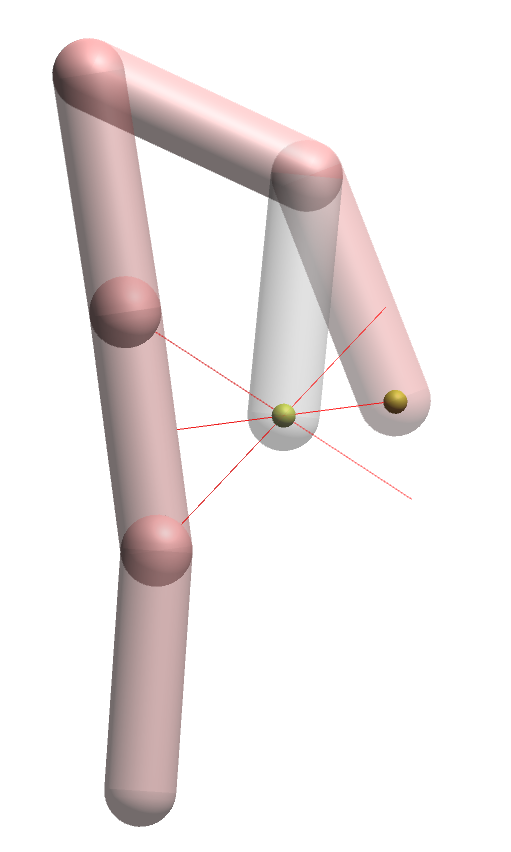
\includegraphics[width=\textwidth]{Figures/simple_distortion_3.png}
        \caption{$\gamma = 3$}
    \end{subfigure}
    ~ %add desired spacing between images, e. g. ~, \quad, \qquad, \hfill etc.
    %(or a blank line to force the subfigure onto a new line)
    \begin{subfigure}[b]{0.2\textwidth}
        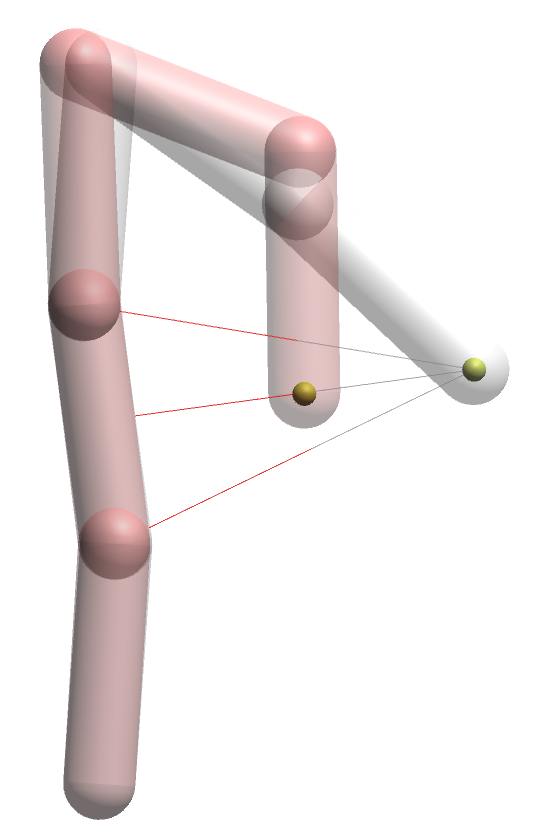
\includegraphics[width=\textwidth]{Figures/simple_distortion_-3.png}
        \caption{$\gamma = -3$}
    \end{subfigure}
    \caption{Two examples of our linear distortion applied to a simple IK arm with multiple segments. The gray lines are the relative displacement vectors and the red ones are their distorted counterparts. Similarly, the gray arms represent the pose the real arm would take whereas the red ones show the two resulting distorted poses.}
    \label{fig:armExamples}
\end{figure}

We will now describe the function we will be using in our subsequent experiment, and then propose a distortion expression that may be better-suited for real-world applications.

\subsection{Linear Function}

For ease of experimentation and understandability, we are looking for a linear function $f(x) = ax + b$. Figure \ref{fig:armExamples} gives an example of what we aim to achieve, while Figure \ref{fig:plotsOfGamma} below gives a more mathematical point of view of the distortion we are looking for, especially in terms of $a$, the slope of the function. This plot, as well as all of the other plots of this report, were obtained using the Plotly API \cite{plotly}.

\begin{figure}[h]
    \center{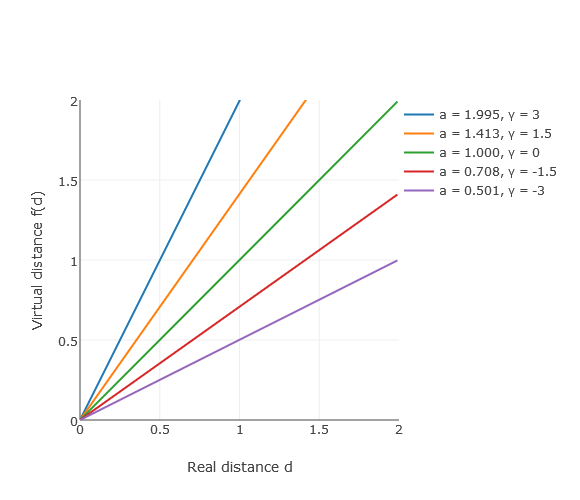
\includegraphics[width=.7\textwidth]
    {Figures/gamma_values.png}}
    \caption{An example of a few distortion functions for various values of slope $a$ and gain $\gamma $.}\label{fig:plotsOfGamma}
\end{figure}

First of all we want to preserve self-haptic contacts. Such contact happens when a relative displacement vector satisfies $\norm{\vec{v}} = 0$, which means that we need $f(0) = 0$, and thus $b = 0$.

Intuitively, the slopes should be arranged around $a=1$, which results in no distortion at all and that we want to correspond to $\gamma = 0$. One can also figure out that there is a correspondence between slopes above and below the line $f(x) = x$. For instance, for a given virtual distance to cover, a slope of \num{0.5} makes the traveling distance twice as long, whereas a slope of \num{2} halves the required movement.

Formally, we are modifying each relative displacement vector as specified in Equation \ref{eq:DistortionOperation}, with $\gamma$ representing a gain, measured in \SI{}{\decibel}, and $f$ defined by Equation \ref{eq:DistortionFunction} below.

\begin{equation}
\label{eq:DistortionFunction}
D(\vec{v},\gamma ) = \hat{\vec{v}} \cdot \norm{\vec{v}} \cdot 10^{\frac{\gamma}{10}}
\end{equation}

In this equation, $\vec{v}$ is a vector, $\hat{\vec{v}}$ is its normalized counterpart, and $\gamma \in \mathbb{R}$. The last factor, $10^{\frac{\gamma}{10}}$, comes from the definition of a gain, in \SI{}{\decibel} \cite{book:decibel}, based on two values $P_1$ and $P_2$ of a single, yet undefined unit:

\begin{align*}
    \text{gain} = \gamma &= 10 \cdot \log_{10} (\frac{P_1}{P_2})\\
    \frac{\gamma}{10} &= \log_{10} (\text{slope})\\
    \text{slope} &= 10^{\frac{\gamma}{10}}.
\end{align*}

A value of $\gamma = 3$ thus indicates that the virtual movement will roughly be twice the amplitude of the registered one ($1.995 \approx 2$), while a gain of $\gamma = -3$ means one will have to travel twice as big a distance (\num{0.501}) as perceived in order to cover it. Figure \ref{fig:armExamples} shows two examples of distortion, and Figure \ref{fig:plotsOfGamma} gives a few instances of this linear distortion functions with varying values of $\gamma $ and the corresponding slope $a$.

\subsection{Other Functions}
\label{sec:otherFunctions}
Before deciding to use a simpler, thus easier to quantify, linear function for our experimentation process, we tried out different functions that we think are of interest for further applications. Two of these functions are described here as a reference for further investigation.

As for our linear function, we require the distortion to be null around $\norm{\vec{v}} = 0$. Similarly, we introduce an action range $a_r$ after which the distortion should be null again. The general form of the function applied to our relative displacement vectors then becomes the one described in Equation \ref{eq:distortionCase}.

\begin{equation}
    \label{eq:distortionCase}
    D(\vec{v}, s, a_r) =
    \begin{cases}
        \hat{v} \cdot \norm{\vec{v}} \cdot f(\norm{\vec{v}}, s, a_r)    &\text{if } \norm{\vec{v}} \leq a_r\\
        \vec{v}                                                         &\text{otherwise}
    \end{cases}
\end{equation}

Note that we changed the `$\gamma $' parameter for `$s$', which is due to this parameter no longer denoting a cleanly defined gain, but a vaguer concept of strength. Two notable instances of the function $f$ were implemented. They are shown in Figure \ref{fig:otherDistortions} and are described hereafter.

\begin{figure}[h]
    \centering
    \begin{subfigure}[b]{.45\textwidth}
        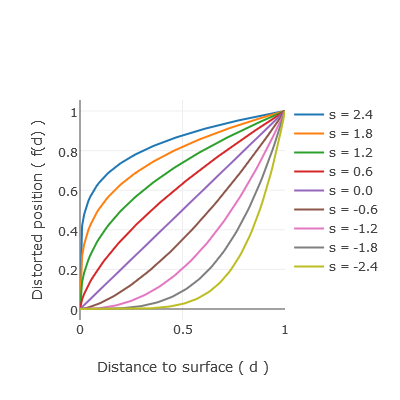
\includegraphics[width=\textwidth]{Figures/exponential_distortion.png}
        \caption{Exponential}
        \label{fig:otherDistortionsExp}
    \end{subfigure}
    ~
    \begin{subfigure}[b]{.45\textwidth}
        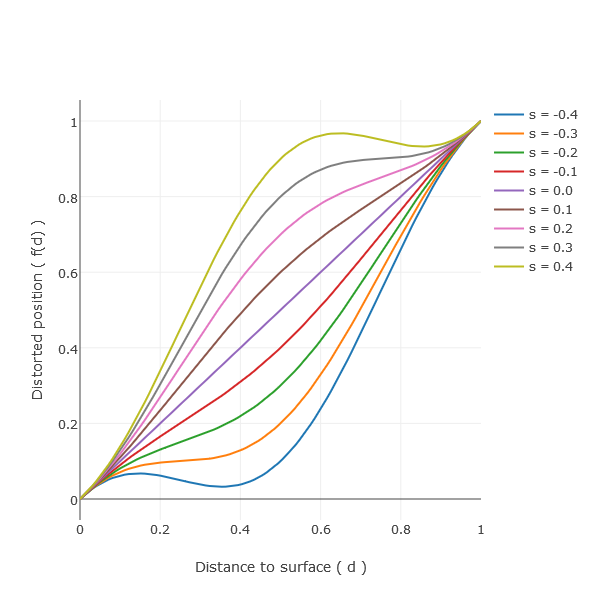
\includegraphics[width=\textwidth]{Figures/cosine_distortion.png}
        \caption{Cosine}
        \label{fig:otherDistortionsCos}
    \end{subfigure}
    \caption{Multiple instances of the two alternative distortion functions we propose in section \ref{sec:otherFunctions}. Both have been plotted using $a_r = 1$, only varying the strength parameter $s$.}
    \label{fig:otherDistortions}
\end{figure}

\subsubsection{Exponential}

Based on an expression proposed by Khoury \cite{khoury2015human}, this function has the following form:

\begin{equation*}
    f(d, a_r, s) = a_r \cdot \Bigg(\frac{d}{a_r}\Bigg)^{2^{-s}}
\end{equation*}

As one can observe on Figure \ref{fig:otherDistortions}, this function has the advantage of smoothly transitioning from a non-distorted position to a maximum discrepancy, and then back to an undistorted position around $d=a_r$.

More observations on the exponential function, particularly on the high velocity discrepancy around the ends of the distorted range.

\subsubsection{Cosine}

Observations made on the previous function lead us to designing this second function.

\begin{equation*}
    f(d, a_r, s) = \frac{s}{2}\Bigg(1 - \cos\Big(\frac{2\pi}{a_r} \cdot d\Big)\Bigg) + d
\end{equation*}

Obviously, being smoother in terms of velocity near both ends of the distorted area leads to trade-offs. In our case the function introduces higher velocity discrepancies at other locations, as one can observe on Figure \ref{fig:otherDistortionsCos}. At higher strengths (e.g.\ $s=0.4$) the function even forces the virtual hand to go backwards in order to rejoin the real position before approaching $a_r$.

\section{Egocentric Normalization Factor}

We added one more modification to the definition of the position proposed by \cite{molla2017egocentric} which we modified to obtain Equation \ref{eq:DistortionOperation}, and more precisely the way $\lambda $ is defined. As originally explained by \cite{molla2016precise} as well as in Section \ref{sec:egocentric}, it is computed as the product of two importance factors, proximity and orthogonality, respectively denoted $\lambda_p$ and $\lambda_\perp $.

The former importance factor was initially defined as $\lambda_p = \frac{1}{\norm{\vec{v}}}$. In practice we find that this formula does not give enough importance to nearby body parts, and we decided to change it slightly as $\lambda_p = \frac{1}{\norm{\vec{v}}^2}$. --Mention angle solide.-- % which more closely represents the amount of surface of an object that is visible at a distance $\norm{\vec{v}}$.

\section{Reachable Sphere}

A few words on the concept of reachable sphere and how it might help at the limits of the reachable space.
